\begin{figure}
\centering

\begin{subfigure}[b]{0.25\columnwidth}
\centering
\cfbox{box-gray}{
\resizebox{!}{\textwidth}{
\tikzsetnextfilename{model1_1}
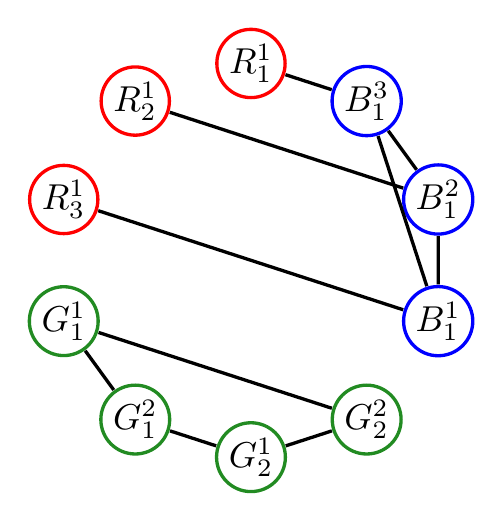
\begin{tikzpicture}[
mynode/.style={draw, circle, very thick, inner sep=1pt, scale=1.3},
myline/.style={draw, very thick},
]
\pgfmathsetmacro{\n}{10};
\pgfmathsetmacro{\r}{2.5};

\node[mynode,draw=red] (1) at (0*360/\n + 90: \r cm) {$\xcolor{R}_1^1$};
\node[mynode,draw=red] (2) at (1*360/\n + 90: \r cm) {$\xcolor{R}_2^1$};
\node[mynode,draw=red] (3) at  (2*360/\n + 90: \r cm) {$\xcolor{R}_3^1$};
\node[mynode,draw=ForestGreen] (4) at  (3*360/\n + 90: \r cm) {$\xcolor{G}_1^1$};
\node[mynode,draw=ForestGreen] (5) at  (4*360/\n + 90: \r cm) {$\xcolor{G}_1^2$};
\node[mynode,draw=ForestGreen] (6) at  (5*360/\n + 90: \r cm) {$\xcolor{G}_2^1$};
\node[mynode,draw=ForestGreen] (7) at  (6*360/\n + 90: \r cm) {$\xcolor{G}_2^2$};
\node[mynode,draw=blue] (8) at  (7*360/\n + 90: \r cm) {$\xcolor{B}_1^1$};
\node[mynode,draw=blue] (9) at  (8*360/\n + 90: \r cm) {$\xcolor{B}_1^2$};
\node[mynode,draw=blue] (10) at  (9*360/\n + 90: \r cm) {$\xcolor{B}_1^3$};


\draw [myline] (10) -- (1);
\draw [myline] (9) -- (2);
\draw [myline] (8) -- (3);
\draw [myline] (7) -- (4);
\draw [myline] (6) -- (5);

\draw [myline] (4) -- (5);
\draw [myline] (6) -- (7);
\draw [myline] (8) -- (9);
\draw [myline] (8) -- (10);
\draw [myline] (9) -- (10);

\end{tikzpicture}
}
}
\caption{$G^{CP}$  for  \mypm{}~1.\label{fig:ch2:model1_1}}
\end{subfigure}
%
% \hspace{0.02\textwidth}
%
\begin{subfigure}[b]{0.25\columnwidth}
\centering
\cfbox{box-gray}{
\resizebox{!}{\textwidth}{
\tikzsetnextfilename{model1_2}
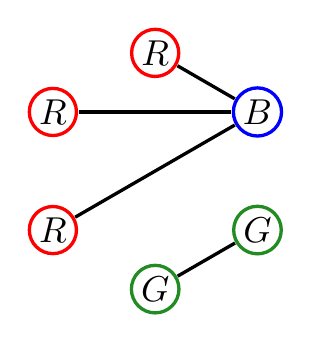
\begin{tikzpicture}[
mynode/.style={draw, circle, very thick, inner sep=1pt, scale=1.3},
myline/.style={draw, very thick},
]
\pgfmathsetmacro{\n}{6};
\pgfmathsetmacro{\r}{1.5};

\node[mynode,draw=red] (1) at (0*360/\n + 90: \r cm) {$\xcolor{R}$};
\node[mynode,draw=red] (2) at (1*360/\n + 90: \r cm) {$\xcolor{R}$};
\node[mynode,draw=red] (3) at  (2*360/\n + 90: \r cm) {$\xcolor{R}$};
\node[mynode,draw=ForestGreen] (4) at  (3*360/\n + 90: \r cm) {$\xcolor{G}$};
\node[mynode,draw=ForestGreen] (5) at  (4*360/\n + 90: \r cm) {$\xcolor{G}$};
\node[mynode,draw=blue, circle] (6) at  (5*360/\n + 90: \r cm) {$\xcolor{B}$};

\draw [myline] (1) -- (6);
\draw [myline] (2) -- (6);
\draw [myline] (3) -- (6);
\draw [myline] (4) -- (5);

\end{tikzpicture}
}
}
\caption{$G^{CC}$  for  \mypm{}~1.\label{fig:ch2:model1_2}}
\end{subfigure}
%
% \hspace{0.02\textwidth}
%
%\begin{subfigure}[b]{0.32\columnwidth}
%\centering
%\cfbox{box-gray}{
%\resizebox{!}{\textwidth}{
%\tikzsetnextfilename{model1_3}
%\begin{tikzpicture}[
%mynode/.style={draw, circle, very thick, inner sep=1pt, scale=1.3},
%myline/.style={draw, very thick},
%]
%\pgfmathsetmacro{\n}{10};
%\pgfmathsetmacro{\r}{2.5};
%
%\node[mynode,draw=red] (1) at (0*360/\n + 90: \r cm) {$\xcolor{R}_1^1$};
%\node[mynode,draw=red] (2) at (1*360/\n + 90: \r cm) {$\xcolor{R}_2^1$};
%\node[mynode,draw=red] (3) at  (2*360/\n + 90: \r cm) {$\xcolor{R}_3^1$};
%\node[mynode,draw=ForestGreen] (4) at  (3*360/\n + 90: \r cm) {$\xcolor{G}_1^1$};
%\node[mynode,draw=ForestGreen] (5) at  (4*360/\n + 90: \r cm) {$\xcolor{G}_1^2$};
%\node[mynode,draw=ForestGreen] (6) at  (5*360/\n + 90: \r cm) {$\xcolor{G}_2^1$};
%\node[mynode,draw=ForestGreen] (7) at  (6*360/\n + 90: \r cm) {$\xcolor{G}_2^2$};
%\node[mynode,draw=blue] (8) at  (7*360/\n + 90: \r cm) {$\xcolor{B}_1^1$};
%\node[mynode,draw=blue] (9) at  (8*360/\n + 90: \r cm) {$\xcolor{B}_1^2$};
%\node[mynode,draw=blue] (10) at  (9*360/\n + 90: \r cm) {$\xcolor{B}_1^3$};
%
%
%\draw [myline] (10) -- (5);
%\draw [myline] (9) -- (3);
%\draw [myline] (8) -- (6);
%\draw [myline] (7) -- (4);
%\draw [myline] (2) -- (1);
%
%\draw [myline] (4) -- (5);
%\draw [myline] (6) -- (7);
%\draw [myline] (8) -- (9);
%\draw [myline] (8) -- (10);
%\draw [myline] (9) -- (10);
%
%\end{tikzpicture}
%}
%}
%\caption{$G^{CP}$  for  \mypm{}~462.\label{fig:model1_3}}
%\end{subfigure}
%%
%\hspace{0.02\textwidth}
%%
\begin{subfigure}[b]{0.25\columnwidth}
\centering
\cfbox{box-gray}{
\resizebox{!}{\textwidth}{
\tikzsetnextfilename{model1_4}
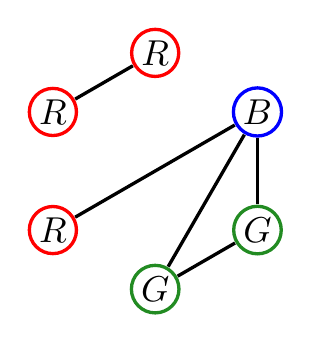
\begin{tikzpicture}[
mynode/.style={draw, circle, very thick, inner sep=1pt, scale=1.3},
myline/.style={draw, very thick},
]
\pgfmathsetmacro{\n}{6};
\pgfmathsetmacro{\r}{1.5};

\node[mynode,draw=red] (1) at (0*360/\n + 90: \r cm) {$\xcolor{R}$};
\node[mynode,draw=red] (2) at (1*360/\n + 90: \r cm) {$\xcolor{R}$};
\node[mynode,draw=red] (3) at  (2*360/\n + 90: \r cm) {$\xcolor{R}$};
\node[mynode,draw=ForestGreen] (4) at  (3*360/\n + 90: \r cm) {$\xcolor{G}$};
\node[mynode,draw=ForestGreen] (5) at  (4*360/\n + 90: \r cm) {$\xcolor{G}$};
\node[mynode,draw=blue, circle] (6) at  (5*360/\n + 90: \r cm) {$\xcolor{B}$};

\draw [myline] (1) -- (2);
\draw [myline] (3) -- (6);
\draw [myline] (4) -- (6);
\draw [myline] (5) -- (6);
\draw [myline] (5) -- (4);

\end{tikzpicture}
}
}
\caption{$G^{CC}$ for \mypm{}~462.\label{fig:ch2:model1_4}}
\end{subfigure}

\caption{Select connected ports and connected component graphs for \nameref{sec:ch2:example1}.\label{fig:model1}}

\end{figure}